\documentclass[10pt]{article}
\usepackage{fontspec}
\usepackage{amsmath}
\usepackage{unicode-math}
\usepackage{amsthm}
\usepackage{graphicx}
\usepackage{tikz}
\usepackage{setspace}
\usepackage{algorithm}
\usepackage{algpseudocode}
\usetikzlibrary{arrows.meta}
\usetikzlibrary{positioning}
\usetikzlibrary{shapes.geometric}

\def\OPTpagesize{210mm,297mm}

\usepackage[papersize={\OPTpagesize},
            twoside=false,
            includehead=true,
            top=0.5in,
            bottom=0.5in,
            left=0.5in,
            right=0.5in]{geometry}
\usepackage{fancyhdr}

\pagestyle{fancy}
\setlength{\headheight}{15pt}
\lhead{Homework 4}
\rhead{\thepage}
\cfoot{}
\lfoot{}
\rfoot{}
\setlength{\parindent}{0mm}
\setstretch{1.2}

\def\checkmark{\tikz\fill[scale=0.4](0,.35) -- (.25,0) -- (1,.7) -- (.25,.15) -- cycle;}

\begin{document}
\title{Homework 4}
\author{Zhengyang Ling}
\maketitle
\thispagestyle{fancy}
\section{}
\paragraph{}(improve)
\subparagraph{}
For improve agent, we use the neural network to reconize the color.
Initially, our neural network structure look like this
\begin{center}
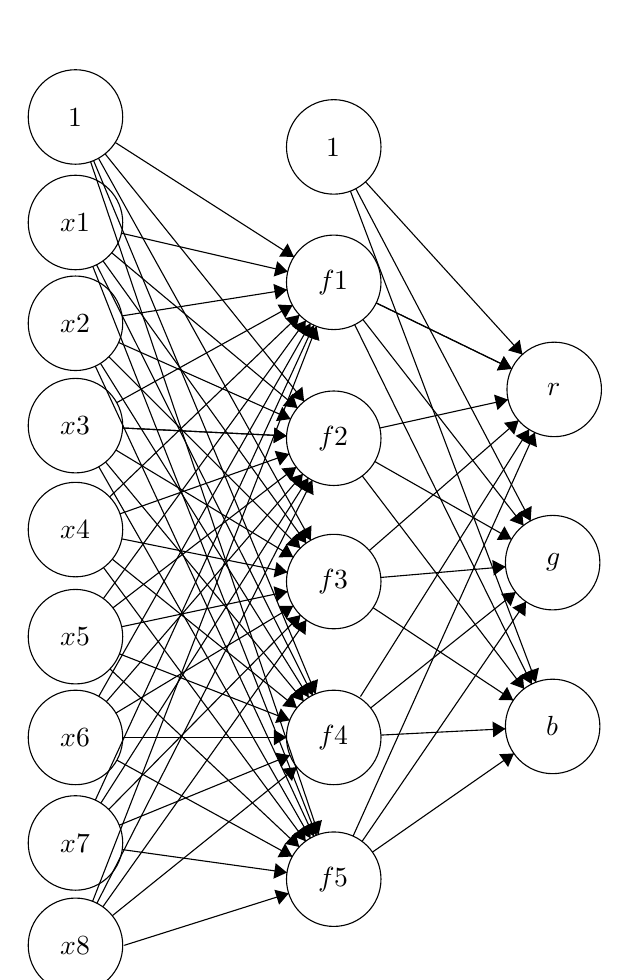
\begin{tikzpicture}[scale=0.2]
\tikzstyle{every node}+=[inner sep=0pt]
\draw [black] (20.4,-23.8) circle (3);
\draw (20.4,-23.8) node {$x3$};
\draw [black] (20.4,-17.3) circle (3);
\draw (20.4,-17.3) node {$x2$};
\draw [black] (20.4,-30.4) circle (3);
\draw (20.4,-30.4) node {$x4$};
\draw [black] (20.4,-37.2) circle (3);
\draw (20.4,-37.2) node {$x5$};
\draw [black] (20.4,-43.6) circle (3);
\draw (20.4,-43.6) node {$x6$};
\draw [black] (20.4,-10.9) circle (3);
\draw (20.4,-10.9) node {$x1$};
\draw [black] (20.4,-50.3) circle (3);
\draw (20.4,-50.3) node {$x7$};
\draw [black] (20.4,-56.8) circle (3);
\draw (20.4,-56.8) node {$x8$};
\draw [black] (20.4,-4.2) circle (3);
\draw (20.4,-4.2) node {$1$};
\draw [black] (36.8,-14.7) circle (3);
\draw (36.8,-14.7) node {$f1$};
\draw [black] (36.8,-24.6) circle (3);
\draw (36.8,-24.6) node {$f2$};
\draw [black] (36.8,-33.7) circle (3);
\draw (36.8,-33.7) node {$f3$};
\draw [black] (36.8,-43.6) circle (3);
\draw (36.8,-43.6) node {$f4$};
\draw [black] (36.8,-52.6) circle (3);
\draw (36.8,-52.6) node {$f5$};
\draw [black] (36.8,-6.1) circle (3);
\draw (36.8,-6.1) node {$1$};
\draw [black] (50.8,-21.5) circle (3);
\draw (50.8,-21.5) node {$r$};
\draw [black] (50.7,-32.5) circle (3);
\draw (50.7,-32.5) node {$g$};
\draw [black] (50.7,-42.9) circle (3);
\draw (50.7,-42.9) node {$b$};
\draw [black] (22.93,-5.82) -- (34.27,-13.08);
\fill [black] (34.27,-13.08) -- (33.87,-12.23) -- (33.33,-13.07);
\draw [black] (23.32,-11.58) -- (33.88,-14.02);
\fill [black] (33.88,-14.02) -- (33.21,-13.36) -- (32.99,-14.33);
\draw [black] (23.36,-16.83) -- (33.84,-15.17);
\fill [black] (33.84,-15.17) -- (32.97,-14.8) -- (33.13,-15.79);
\draw [black] (23.02,-22.34) -- (34.18,-16.16);
\fill [black] (34.18,-16.16) -- (33.23,-16.11) -- (33.72,-16.98);
\draw [black] (22.57,-28.33) -- (34.63,-16.77);
\fill [black] (34.63,-16.77) -- (33.71,-16.97) -- (34.4,-17.69);
\draw [black] (22.17,-34.78) -- (35.03,-17.12);
\fill [black] (35.03,-17.12) -- (34.16,-17.48) -- (34.97,-18.07);
\draw [black] (21.88,-40.99) -- (35.32,-17.31);
\fill [black] (35.32,-17.31) -- (34.49,-17.76) -- (35.36,-18.25);
\draw [black] (21.66,-47.58) -- (35.54,-17.42);
\fill [black] (35.54,-17.42) -- (34.76,-17.94) -- (35.66,-18.36);
\draw [black] (21.49,-54) -- (35.71,-17.5);
\fill [black] (35.71,-17.5) -- (34.95,-18.06) -- (35.89,-18.42);
\draw [black] (22.28,-6.54) -- (34.92,-22.26);
\fill [black] (34.92,-22.26) -- (34.81,-21.33) -- (34.03,-21.95);
\draw [black] (22.7,-12.82) -- (34.5,-22.68);
\fill [black] (34.5,-22.68) -- (34.2,-21.78) -- (33.56,-22.55);
\draw [black] (23.14,-18.52) -- (34.06,-23.38);
\fill [black] (34.06,-23.38) -- (33.53,-22.6) -- (33.13,-23.51);
\draw [black] (23.4,-23.95) -- (33.8,-24.45);
\fill [black] (33.8,-24.45) -- (33.03,-23.92) -- (32.98,-24.91);
\draw [black] (23.4,-23.95) -- (33.8,-24.45);
\fill [black] (33.8,-24.45) -- (33.03,-23.92) -- (32.98,-24.91);
\draw [black] (23.23,-29.4) -- (33.97,-25.6);
\fill [black] (33.97,-25.6) -- (33.05,-25.4) -- (33.38,-26.34);
\draw [black] (22.78,-35.37) -- (34.42,-26.43);
\fill [black] (34.42,-26.43) -- (33.48,-26.52) -- (34.09,-27.31);
\draw [black] (22.36,-41.33) -- (34.84,-26.87);
\fill [black] (34.84,-26.87) -- (33.94,-27.15) -- (34.7,-27.8);
\draw [black] (22.01,-47.77) -- (35.19,-27.13);
\fill [black] (35.19,-27.13) -- (34.33,-27.53) -- (35.18,-28.07);
\draw [black] (21.76,-54.13) -- (35.44,-27.27);
\fill [black] (35.44,-27.27) -- (34.63,-27.76) -- (35.52,-28.21);
\draw [black] (21.86,-6.82) -- (35.34,-31.08);
\fill [black] (35.34,-31.08) -- (35.39,-30.14) -- (34.52,-30.62);
\draw [black] (21.55,-6.97) -- (35.65,-40.83);
\fill [black] (35.65,-40.83) -- (35.8,-39.9) -- (34.88,-40.28);
\draw [black] (21.36,-7.04) -- (35.84,-49.76);
\fill [black] (35.84,-49.76) -- (36.05,-48.84) -- (35.11,-49.16);
\draw [black] (22.15,-13.34) -- (35.05,-31.26);
\fill [black] (35.05,-31.26) -- (34.99,-30.32) -- (34.18,-30.91);
\draw [black] (21.74,-13.58) -- (35.46,-40.92);
\fill [black] (35.46,-40.92) -- (35.54,-39.98) -- (34.65,-40.43);
\draw [black] (21.5,-13.69) -- (35.7,-49.81);
\fill [black] (35.7,-49.81) -- (35.87,-48.88) -- (34.94,-49.25);
\draw [black] (22.52,-19.42) -- (34.68,-31.58);
\fill [black] (34.68,-31.58) -- (34.47,-30.66) -- (33.76,-31.37);
\draw [black] (21.99,-19.85) -- (35.21,-41.05);
\fill [black] (35.21,-41.05) -- (35.21,-40.11) -- (34.37,-40.64);
\draw [black] (21.66,-20.02) -- (35.54,-49.88);
\fill [black] (35.54,-49.88) -- (35.65,-48.94) -- (34.75,-49.36);
\draw [black] (22.97,-25.35) -- (34.23,-32.15);
\fill [black] (34.23,-32.15) -- (33.81,-31.31) -- (33.29,-32.16);
\draw [black] (22.31,-26.11) -- (34.89,-41.29);
\fill [black] (34.89,-41.29) -- (34.76,-40.35) -- (33.99,-40.99);
\draw [black] (21.88,-26.41) -- (35.32,-49.99);
\fill [black] (35.32,-49.99) -- (35.35,-49.05) -- (34.49,-49.55);
\draw [black] (23.34,-30.99) -- (33.86,-33.11);
\fill [black] (33.86,-33.11) -- (33.17,-32.46) -- (32.98,-33.44);
\draw [black] (22.74,-32.28) -- (34.46,-41.72);
\fill [black] (34.46,-41.72) -- (34.15,-40.83) -- (33.53,-41.61);
\draw [black] (22.18,-32.81) -- (35.02,-50.19);
\fill [black] (35.02,-50.19) -- (34.94,-49.25) -- (34.14,-49.84);
\draw [black] (23.33,-36.57) -- (33.87,-34.33);
\fill [black] (33.87,-34.33) -- (32.98,-34) -- (33.19,-34.98);
\draw [black] (23.19,-38.29) -- (34.01,-42.51);
\fill [black] (34.01,-42.51) -- (33.44,-41.75) -- (33.08,-42.68);
\draw [black] (23.03,-45.04) -- (34.17,-51.16);
\fill [black] (34.17,-51.16) -- (33.71,-50.33) -- (33.23,-51.21);
\draw [black] (22.59,-39.25) -- (34.61,-50.55);
\fill [black] (34.61,-50.55) -- (34.37,-49.63) -- (33.69,-50.36);
\draw [black] (22.97,-42.05) -- (34.23,-35.25);
\fill [black] (34.23,-35.25) -- (33.29,-35.24) -- (33.81,-36.09);
\draw [black] (23.4,-43.6) -- (33.8,-43.6);
\fill [black] (33.8,-43.6) -- (33,-43.1) -- (33,-44.1);
\draw [black] (22.51,-48.17) -- (34.69,-35.83);
\fill [black] (34.69,-35.83) -- (33.77,-36.05) -- (34.49,-36.75);
\draw [black] (23.18,-49.17) -- (34.02,-44.73);
\fill [black] (34.02,-44.73) -- (33.09,-44.57) -- (33.47,-45.5);
\draw [black] (23.37,-50.72) -- (33.83,-52.18);
\fill [black] (33.83,-52.18) -- (33.11,-51.58) -- (32.97,-52.57);
\draw [black] (22.14,-54.35) -- (35.06,-36.15);
\fill [black] (35.06,-36.15) -- (34.19,-36.51) -- (35.01,-37.09);
\draw [black] (22.74,-54.92) -- (34.46,-45.48);
\fill [black] (34.46,-45.48) -- (33.53,-45.59) -- (34.15,-46.37);
\draw [black] (23.5,-56.8) -- (33.94,-53.5);
\fill [black] (33.94,-53.5) -- (33.03,-53.27) -- (33.33,-54.22);
\draw [black] (39.5,-16.01) -- (48.1,-20.19);
\fill [black] (48.1,-20.19) -- (47.6,-19.39) -- (47.16,-20.29);
\draw [black] (39.73,-23.95) -- (47.87,-22.15);
\fill [black] (47.87,-22.15) -- (46.98,-21.83) -- (47.2,-22.81);
\draw [black] (39.06,-31.73) -- (48.54,-23.47);
\fill [black] (48.54,-23.47) -- (47.61,-23.62) -- (48.26,-24.37);
\draw [black] (38.5,-41) -- (49.2,-24.04);
\fill [black] (49.2,-24.04) -- (48.35,-24.45) -- (49.2,-24.98);
\draw [black] (38.03,-49.86) -- (49.57,-24.24);
\fill [black] (49.57,-24.24) -- (48.78,-24.76) -- (49.7,-25.17);
\draw [black] (38.82,-8.32) -- (48.78,-19.28);
\fill [black] (48.78,-19.28) -- (48.61,-18.35) -- (47.87,-19.02);
\draw [black] (38.2,-8.75) -- (49.3,-29.85);
\fill [black] (49.3,-29.85) -- (49.37,-28.9) -- (48.49,-29.37);
\draw [black] (37.86,-8.91) -- (49.64,-40.09);
\fill [black] (49.64,-40.09) -- (49.83,-39.17) -- (48.89,-39.52);
\draw [black] (39.5,-16.01) -- (48.1,-20.19);
\fill [black] (48.1,-20.19) -- (47.6,-19.39) -- (47.16,-20.29);
\draw [black] (38.65,-17.06) -- (48.85,-30.14);
\fill [black] (48.85,-30.14) -- (48.76,-29.2) -- (47.97,-29.81);
\draw [black] (38.13,-17.39) -- (49.37,-40.21);
\fill [black] (49.37,-40.21) -- (49.47,-39.27) -- (48.57,-39.71);
\draw [black] (39.41,-26.08) -- (48.09,-31.02);
\fill [black] (48.09,-31.02) -- (47.64,-30.19) -- (47.15,-31.06);
\draw [black] (38.61,-26.99) -- (48.89,-40.51);
\fill [black] (48.89,-40.51) -- (48.8,-39.57) -- (48,-40.18);
\draw [black] (39.79,-33.44) -- (47.71,-32.76);
\fill [black] (47.71,-32.76) -- (46.87,-32.33) -- (46.96,-33.32);
\draw [black] (39.3,-35.36) -- (48.2,-41.24);
\fill [black] (48.2,-41.24) -- (47.81,-40.39) -- (47.26,-41.22);
\draw [black] (39.14,-41.73) -- (48.36,-34.37);
\fill [black] (48.36,-34.37) -- (47.42,-34.48) -- (48.04,-35.26);
\draw [black] (39.8,-43.45) -- (47.7,-43.05);
\fill [black] (47.7,-43.05) -- (46.88,-42.59) -- (46.93,-43.59);
\draw [black] (38.6,-50.2) -- (49.01,-34.98);
\fill [black] (49.01,-34.98) -- (48.14,-35.35) -- (48.97,-35.92);
\draw [black] (39.26,-50.88) -- (48.24,-44.62);
\fill [black] (48.24,-44.62) -- (47.3,-44.66) -- (47.87,-45.48);
\end{tikzpicture}
\end{center}
The activation function that we chose is ReLu function.
The result of this is the following graph
  \begin{figure}[h]
    \centering
    \includegraphics*[scale=0.25]{finalz.png}
  \caption{ nn.}
  \end{figure}
\pagebreak
It can understand that the different pixel corresponding to different color.
But it cannot generate the color correctly. Actually, it looks like the result of the linear regression.( our first improve attempt).
\begin{figure}[h]
  \centering
  \includegraphics*[scale=1]{微信图片_20210503102108.png}
\caption{ linear regression }
\end{figure}
\pagebreak
\subparagraph{}
Then, we decided use a larger input to reconstruct the color of pixel. This time we use the 15*15 replace the 3*3. Then, the neural network look like this.
\begin{figure}[h]
  \centering
  \includegraphics*[scale=0.25]{图片1.png}
\caption{ 15*15 }
\end{figure}
\subparagraph{}
However, the result also is not good.It looks like so fuzzy. We think it may because the two adjacent points share the similar environment.
\begin{figure}[h]
  \centering
  \includegraphics*[scale=0.25]{15.png}
\caption{ 15*15 }
\end{figure}
\pagebreak
\subparagraph{}
Thus, we go back to the first neural network. We use k-measn generate 5 representative color and replace the color of the graph that generated by neural network with the closest representative color.
It looks like this.
\begin{figure}[h]
  \centering
  \includegraphics*[scale=0.25]{final+knn.png}
\caption{ with knn }
\end{figure}
\pagebreak
\subparagraph{}
Some detail: we have used the Xavier Initialization in our program, but it generate strange result. Thus, we replace this initial weight with some constant. We have choose ReLu as our activation function because the derivative of ReLu is simple. It can make the Backpropagation become easy. The loss function that we use is $Loss=\sum((f(x)-y)^2)/3$. The corresponding derivative is $-2(f(x)-y_i)/3$. We have tried to transfer the input the rgb to lab format in order to get the better result, but the result is no so good. Thus, we did not do any pre-processing of the input data. In order to avoid the overfit, we reduce the number of sample and use the L1 Regularization. lam is the parament of the Regularization
\begin{figure}[h]
  \centering
  \includegraphics*[scale=0.25]{finalrandomini.png}
\caption{ random }
\end{figure}
\begin{figure}[h]
  \centering
  \includegraphics*[scale=0.25]{微信图片_20210503105547.png}
\caption{ random }
\end{figure}
\begin{figure}[h]
  \centering
  \includegraphics*[scale=0.25]{微信图片_20210503105551.png}
\caption{ random }
\end{figure}
\begin{figure}[h]
  \centering
  \includegraphics*[scale=0.25]{微信图片_20210503105556.png}
\caption{ random }
\end{figure}
\begin{figure}[h]
  \centering
  \includegraphics*[scale=0.25]{微信图片_20210503105559.png}
\caption{ random }
\end{figure}



\end{document}
